\subsection{Resultate}

Es ist an dieser Stelle schwierig eine abschliessende Aussage zu machen. Das Netzwerk wurde mit den Hermitepolynomen als Startparameter für die Burgersgleichung trainiert. Zur Validierung der Resultate können natürlich keine Hermite-Polynome verwendet werden, da der 'Lernerfolg' nicht wirklich ersichtlich ist, wir möchten wissen wie sich das neuronale Netzwerk auf neuem und noch nie gesehenem verhält. Um dies zu testen wurde als Anfangsbedinung $(1 + sin(2x)) / 2$ gewählt. Die Entwicklung wird in Abbildung \ref{fig:mst_burgers_predict_1} verdeutlicht.

\begin{figure}
	\centering
	\begin{tabular}{ccc}
		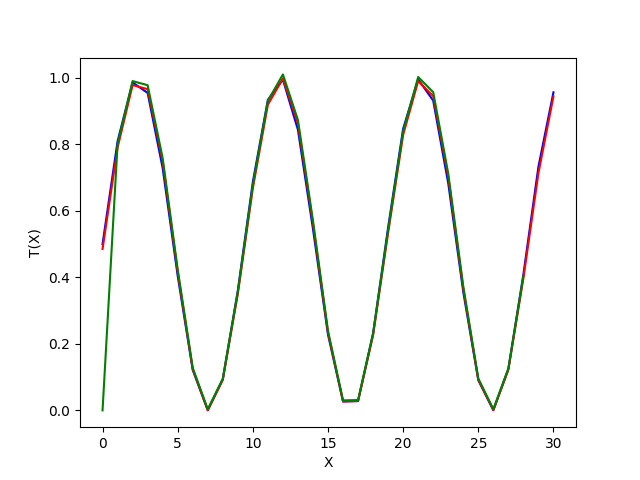
\includegraphics[scale=0.27]{learning/img/burger_predict0.png} &
		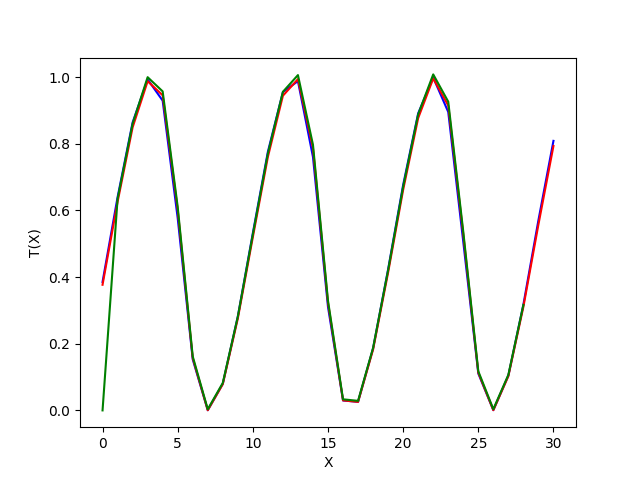
\includegraphics[scale=0.27]{learning/img/burger_predict10.png} &
		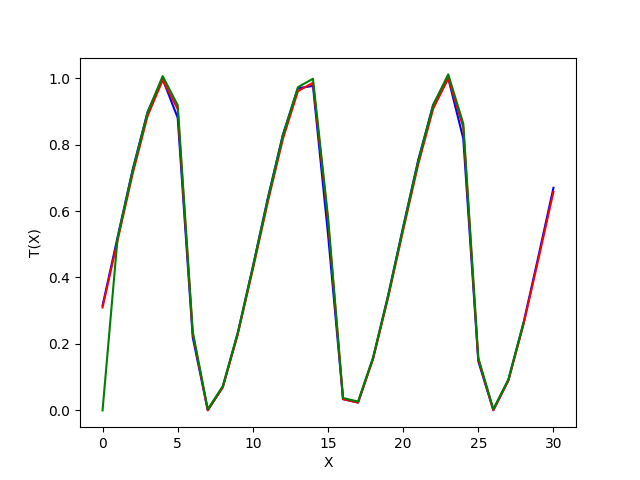
\includegraphics[scale=0.27]{learning/img/burger_predict20.png}
	\end{tabular}
	\label{fig:mst_burgers_predict_1}
	\caption{Das Vorhersagen des nächsten Zeitschrittes scheint gut zu funktionieren. Blau repräsentiert den aktuellen Zustand $i$, rot den berechneten Zustand $i+1$ und grün den vom neuronalen Netzwerk vorhergesagten Zustand $i+1$. }
\end{figure}

Das Experiment scheint soweit sehr gut ausgegangen zu sein, jedoch ist dieser Teil der Burgersgleichung numerisch stabil und kann gut berechnet werden. Interessant wird die Entwicklung erst in dem Moment, in welchem keine Daten mehr erzeugt werden, und das Netzwerk von sich selbst eine Vorhersage treffen muss. Dies ist in Abbildung \ref{fig:mst_burgers_predict_2} ersichtlich.

\begin{figure}
	\centering
	\begin{tabular}{ccc}
		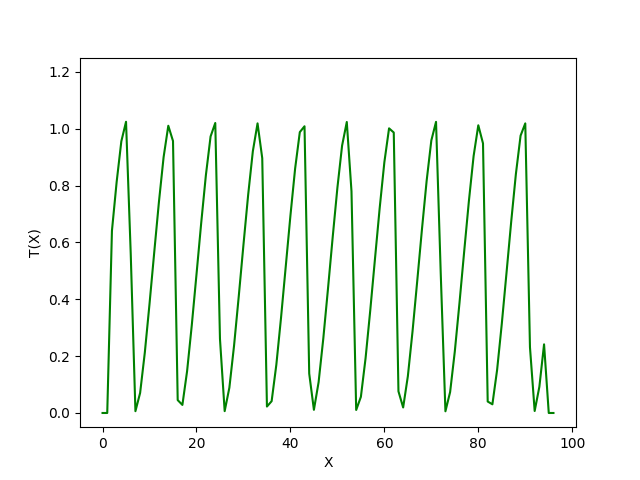
\includegraphics[scale=0.27]{learning/img/burger_predict_full0.png} &
		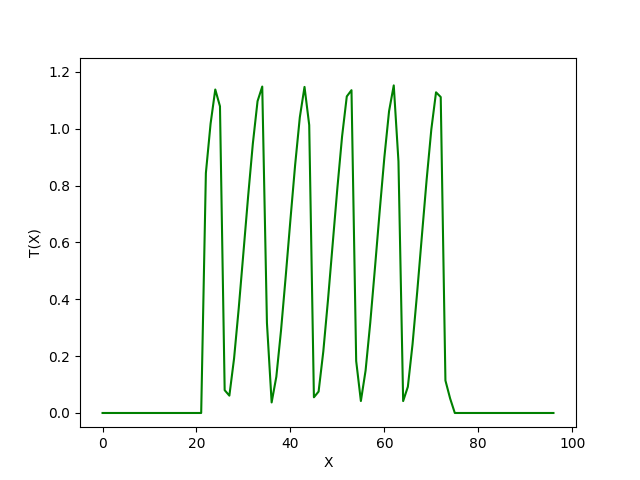
\includegraphics[scale=0.27]{learning/img/burger_predict_full10.png} &
		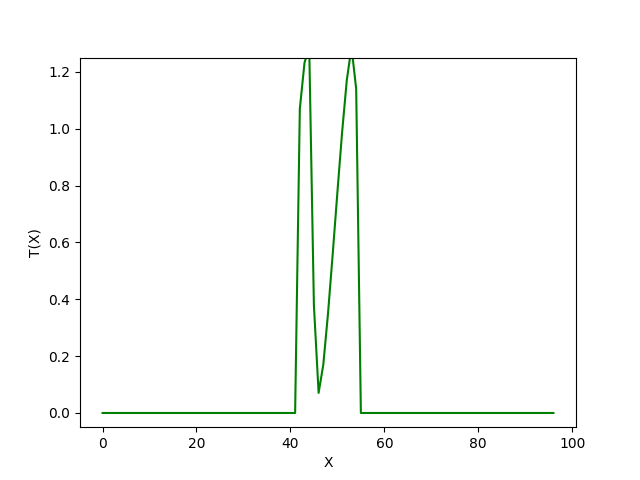
\includegraphics[scale=0.27]{learning/img/burger_predict_full20.png}
	\end{tabular}
	\label{fig:mst_burgers_predict_2}
	\caption{Das Vorhersagen nach der stabilen Phase scheint zu funktionieren, es ist jedoch ersichtlich, dass der Multiplikator nicht ganz perfekt trainiert ist, da ein leichter Anstieg der Maxima von 1 nach 1.25 sattgefunden hat.}
\end{figure}

Auch hier ist zu sehen, dass keine numerischen Instabilitäten entstehen. Das neuronale Netzwerk liefert ebenfals Resutlate welche 'glatt' sind, was weiter aufzeigt, dass dieses Verfahren nicht den numerischen Instabilitäten unterliegt wie andere Methoden. Es ist interessant zu sehen, wie anhand eines sehr einfachen Netzwerks ein Problem trainiert werden kann welches mit numerischen Verfahren nicht so einfach zu lösen ist. Es zeigt ganz klar die Stärke von neuronalen Netzwerken und deren Fähigkeit eine gute Abstraktion zu 'erlernen'.